\documentclass[runningheads]{llncs}
\usepackage[T1]{fontenc}

\usepackage[utf8]{inputenc}
\usepackage{graphicx}
\usepackage[section]{placeins}
\usepackage{float}
\usepackage{url}
\usepackage{orcidlink}
\usepackage{censor}
\usepackage[inline]{enumitem}
\usepackage{framed}

% --- DESABILITAR ANONIMIZAÇÂO ----
%\StopCensoring

\begin{document}

\title{SocialIQA\_pt: A Translation of a Common-Sense Reasoning Dataset about Social Interactions}
\titlerunning{SocialIQA\_pt}
\author{\blackout{Fabio Grassiotto\inst{1}\orcidID{0000-0003-1885-842X} \and
Second Author\inst{2}\orcidID{1111-2222-3333-4444} \and Third Author\inst{3}}}
\authorrunning{\blackout{F. Grassiotto et al.}}
\institute{\blackout{Hub de Inteligência Artificial e Arquiteturas Cognitivas (H.IAAC), Eldorado Research Institute, Campinas- SP, Brazil \and
Institute2 \and Institute3
}}

\maketitle

\begin{abstract}
   Common-sense intelligence, the human ability to apply practical knowledge for everyday decisions, remains a challenging task for AI systems. 
   Datasets like Social IQa, which consist of 38,000 multiple-choice questions to evaluate emotional and social intelligence, are pivotal for advancing AI in this domain. However, such resources are predominantly available in English.
   This paper addresses this gap by presenting a Portuguese language translation of the English dataset Social IQa. Our approach involved using state-of-the-art open-sourced machine translation models, followed by a LLM-driven evaluation method (GEMBA) to rank and select the optimal translations.
   This two-stage methodology ensures high-quality translations, making the dataset accessible for Portuguese-speaking researchers and practitioners, thus promoting advancements in common-sense reasoning and social interactions within the AI community.
\keywords{Machine translation  \and LLM evaluation \and Common-sense reasoning.}
\end{abstract}


\section{Introduction} 

Common-Sense intelligence, usually defined as the human ability of applying
practical knowledge for decisions in everyday life, is still considered a
challenging task for AI systems. As it can be readily perceived when interacting
with chatbots, these systems lack the ability to, through intuition, reason
about common situations and events. Such reasoning requires background knowledge
about how the world works, including the rich nuanced interaction between people
in the social sphere \cite{choi2022curious,krause2023commonsense}.
Therefore, in artificial intelligence, the availability of datasets capable of
benchmarking this task is of utmost importance. Datasets such as Social IQa~\cite{sap2019socialiqa} are readily available in the English language, but we are not aware of any in Portuguese.

The Portuguese language cannot be truly considered a low-resource language as
it is the case with some African and Asian languages, as there are
datasets already available in Portuguese that have millions of tokens. There
are, however, certainly gaps that should be addressed \cite{ghafoor2021impact}.
One of these gaps lies in the availability of datasets that deal with common
sense-reasoning and in special datasets that address social interactions.

This paper presents a two-stage method for creating a Social Intelligence QA dataset in the Portuguese language, derived from the SocialIQa English-language dataset \cite{sap2019socialiqa}. In the first stage, we leverage popular machine translation models available at Hugging Face to generate multiple translation variations for each sentence. In the second stage, we employ a technique of large language model (LLM)-based translation ranking to select the most suitable translation for our Portuguese-language dataset, and provide a comparative analysis of the outcomes from different machine translation models.

This work is structured as follows:
\begin{itemize}
    \item Section 1 \textbf{(this section)}: Here we introduce the work and its motivation.
    \item Section 2 \textbf{Related Work}: We explore the state-of-the-art works related to the field of translation evaluations, both machine and human.
    \item Section 3 \textbf{Dataset}: We describe the SocialIQA original English
    language dataset.
    \item Section 4 \textbf{Methodology}: We describe the translation process
    and the evaluation system we employed.
    \item Section 5 \textbf{Results}: We describe the translated sets results
    and compare them in detail.
    \item Section 6 \textbf{Conclusion and Future Works}: We analyze the results
    we achieved and describe next steps to be taken.
\end{itemize}

\section{Related Work}

The act of evaluating translation output quality is an essential part of machine and/or human-driven translation systems. There were, over the years, a number of proposed techniques that we review here.

\subsection{Human Evaluation Methods}

The best possible assessment of translation quality is still human evaluation. This method usually involves evaluators verifying the translation output to score adequacy and fluency, ranking of translations at the sentence level, and post-editing. Human evaluation is, however, labor intensive and costly. There are also problems with the human evaluation of machine translation: since it is frequently carried out on isolated sentences due to cost issues, inaccuracies tend to rise \cite{freitag2021experts}.

\subsection{Automatic Evaluation Metrics}

Automatic metrics are used as a low-cost alternative to human assessments. They are an invaluable contributor to the development of machine translation, providing automatic feedback during the process \cite{mathur2020tangled}.

The most popular automatic metrics in this field are
\begin{enumerate*}
    \item \textit{BLEU}, BiLingual Evaluation Understudy, that correlates the precision of the n-grams in machine translation output compared to the reference text~\cite{papineni2002bleu}; 
    \item \textit{TER}, Translation Edit Rate, measures the amount of editions required to transform the translated output to the reference~\cite{snover2006study}; 
    \item \textit{chrF}, character n-gram F-score, uses character-level n-grams instead of word n-grams to compare the output with the reference~\cite{popovic2015chrf}; 
    \item \textit{YISI-1}, the romanization of the Cantonese word (‘meaning’), deals with the semantic similarity of the phrases in the output \cite{lo2019yisi}; and 
    \item \textit{ESIM}, Enhanced Sequential Inference Model, is a neural network that, by means of BERT embeddings, computes sentence representations and then compares the similarity to the original text~\cite{chen2016enhanced}.
    
\end{enumerate*}

\subsection{LLM Translation evaluation}

An emerging approach is the usage of large language models to evaluate the quality of machine translation. One of the strengths of LLMs is the support for multilingual questions and answers, what can be used for translation tasks, even if the model has not been trained specifically for this.
Since a model can translate, it should be able to compare translations as well, as can be seen by the work described in \cite{kocmi2023large}.
This paper explores this methodology to create a LLM-ranked translation of a Common-Sense Reasoning dataset, the SocialIQA.


\section{SocialIQA}
The Social Intelligence QA dataset was the first available resource upon its
publication for the measurement of social and emotional intelligence for AI
systems \cite{socialiqa}.
The dataset, collected using a crowd-sourced
framework, is composed of around 38k multiple choice questions, divided into 3
separate bases: development (dev), with 1954 question-answer pairs, training
(train), with 33410 question-answer pairs and test (tst), with 2224
question-answer pairs.

An example of the types of questions and choices can be seen below on Table
\ref{table:SocialIQa}. These are the topmost two rows from the development base
of the dataset.
\begin{table}[!ht]
    \makebox[\textwidth][c]{
        \begin{tabular}{|p{0.9in}|p{0.9in}|p{0.9in}|p{0.9in}|p{0.9in}|p{0.9in}|}\hline
        \textbf{Context}                                                                                                                              & \textbf{Question}                                & \textbf{Answer A}                                                   & \textbf{Answer B}                                                  & \textbf{Answer C}                                            & \textbf{Correct} \\\hline
        Tracy didn't go home that evening and resisted Riley's attacks.                                                                      & What does Tracy need to do before this? & make a new plan                                           & Go home and see Riley                                    & Find somewhere to go                               & C       \\\hline
        Sydney walked past a homeless woman asking for change but did not have any money they could give to her. Sydney felt bad afterwards. & How would you describe Sydney?          & sympathetic                                               & like a person who was unable to help                     & incredulous                                        & A       \\\hline
        Sasha protected the patients' rights by making new laws regarding cancer drug trials.                                                & What will patients want to do next?     & write new laws                                            & get petitions signed                                     & live longer                                        & B       \\\hline
        Jordan was in charge of taking the food on the camping trip and left all the food at home.                                           & How would Jordan feel afterwards?       & horrible that he let his friends down on the camping trip & happy that he doesn't need to do the cooking on the trip & very proud and accomplished about the camping trip & A       \\\hline
        \end{tabular}}
        \caption{Example rows from the SocialIQa English dataset.}\label{table:SocialIQa}
\end{table} 

\section{Methodology} 

Our methodology consisted of two macro-phases, (1) machine translation using
neural network models and (2) comparative evaluation of the translations we
obtained using a large language model. After these macro-phases the best ranked
translation for each row of the dataset was selected for our final dataset.

\subsection{Machine Translation}
\label{subsec:machine-translation}
The first stage of our process, the machine translation stage, aims to execute the translation from English to the Portuguese language. As an input to this stage, the original dataset bases (dev, train, tst) are converted from JSON format to  internal comma-separated files where each one of the sentences is then fed, line by line, to the machine translation models according to prompting prerequisites for each.
The output of this process are again comma-separated files with the translation contents for the dataset bases.

For this work, we selected three machine translation models based on their popularity (amount of downloads) from the Hugging Face website:
\begin{enumerate*}
    \item OPUS-MT project \cite{tiedemann2020opus};
    \item EN-PT translation pre-trained T5 \cite{lopes2020lite}; and
    \item NLLB-200 \cite{costa2022no}.
\end{enumerate*}

\subsubsection{Helsinki-NLP/opus-mt-tc-big-en-pt}

The Helsinki-NLP opus family of models is based on the Marian NMT, an open C++ framework for efficient machine translation developed by the Microsoft Translator team. All these models were converted to Pytorch for hosting at the Hugging Face website.

\subsubsection{unicamp-dl/translation-en-pt-t5}

This model is based on the Text-to-Text Transfer Transformer (T5) pre-trained model with an adaptation to the English tokenizer. According to the literature, the models have a competitive performance to state-of-the-art models while being trained
on modest hardware.

\subsubsection{facebook/nllb-200-distilled-1.3B}

The No Language Left Behind (NLLB) family of models from Meta are primarily intended for research in machine translation, especially for languages with low-resources, allowing for sentence translation among 200 languages.

\subsection{Translation Evaluation}
\label{subsec:translation-evaluation}

The second stage of the proposed method executes a comparison of the quality of the translations obtained on the first step. It takes as input the the comma-separated files with the translation contents, assembles a prompt with the sentences for the three translations requesting a comparison to a large language model and registers the outputs of the evaluation in numerical form. 

We have used this method since there are a number of alternatives for evaluating translations \cite{lee2023survey} and evaluations using large language models have been producing results closer to human evaluation when using LLMs with high complexity (GPT-3.5 turbo and beyond).

GEMBA is one of such methods for quality assessment of translations. The method uses large language models, in particular those available from Open AI, to evaluate the translation of segments of text in isolation by the use of a one-shot prompt system \cite{kocmi2023large}. The three translations were thus compared using this system.

To use GEMBA in this study, we have, however, modified the original prompt. Firstly, we removed the usage of human reference in the evaluation, since we did not have human-curated translations for this set.
Secondly, we changed the prompt to allow for the evaluation of multiple translations at the same time in order to avoid hitting rate limits when using the Open AI APIs.

The modified GEMBA prompt used to query GPT3.5 turbo was:

\begin{framed}
\begin{verbatim}
You are a helpful evaluator of the quality of translations.
Score the following translations from English to Portuguese on a
continuous scale from 0 to 100, where a score of zero means
"no meaning preserved" and score of one hundred means "perfect
meaning and grammar".

En: source_seg
Pt 1: target_seg1
Pt 2: target_seg2
Pt 3: target_seg3
Reply with only the number scores of your evaluation, in a 
python list:
\end{verbatim}
\end{framed}

Where \emph{source\_seg} is the original language group of sentences, and
\emph{target\_seg*} are the proposed translations from each model. GPT-3.5-turbo
replies to this prompt with a Python-style list with the rankings e.g. [80, 85,
100]. Due to optimization issues with using the OpenAI API, the entire dataset
row including the context, question and three answers were bundled together in
the prompt.

\subsection{Workflow}
Our workflow consisted of the five steps described in Figure
\ref{fig:diagram} below. All steps were executed using Python notebook files
available at \cite{socialiqa_pt_impl}.

\begin{itemize}
    \item \textbf{Step I: English dataset conversion} In this step, the original English dataset was converted from JSON format into a temporary  comma-delimited file format for easier processing. 
    \item \textbf{Step II: Machine Translation} In this step, the original
    dataset, available in three separate files for the development, training and testing sets, was translated to the Portuguese language using the three distinct models described in \ref{subsec:machine-translation}.
    \item \textbf{Step III: Translation Evaluation} In this step, translations were evaluated using the evaluation metric GEMBA as described in \ref{subsec:translation-evaluation}.
    \item \textbf{Step IV: Translation selection and ranking} The highest ranked translation set was selected based on the metric described above and used in the dataset.
    \item \textbf{Step V: Portuguese Dataset publishing}  In this step, the
    comma-delimited file with the final translation contents was converted to JSONL format for publishing.
\end{itemize}

\begin{figure}[htbp]
    \centering
    \makebox[\textwidth][c]{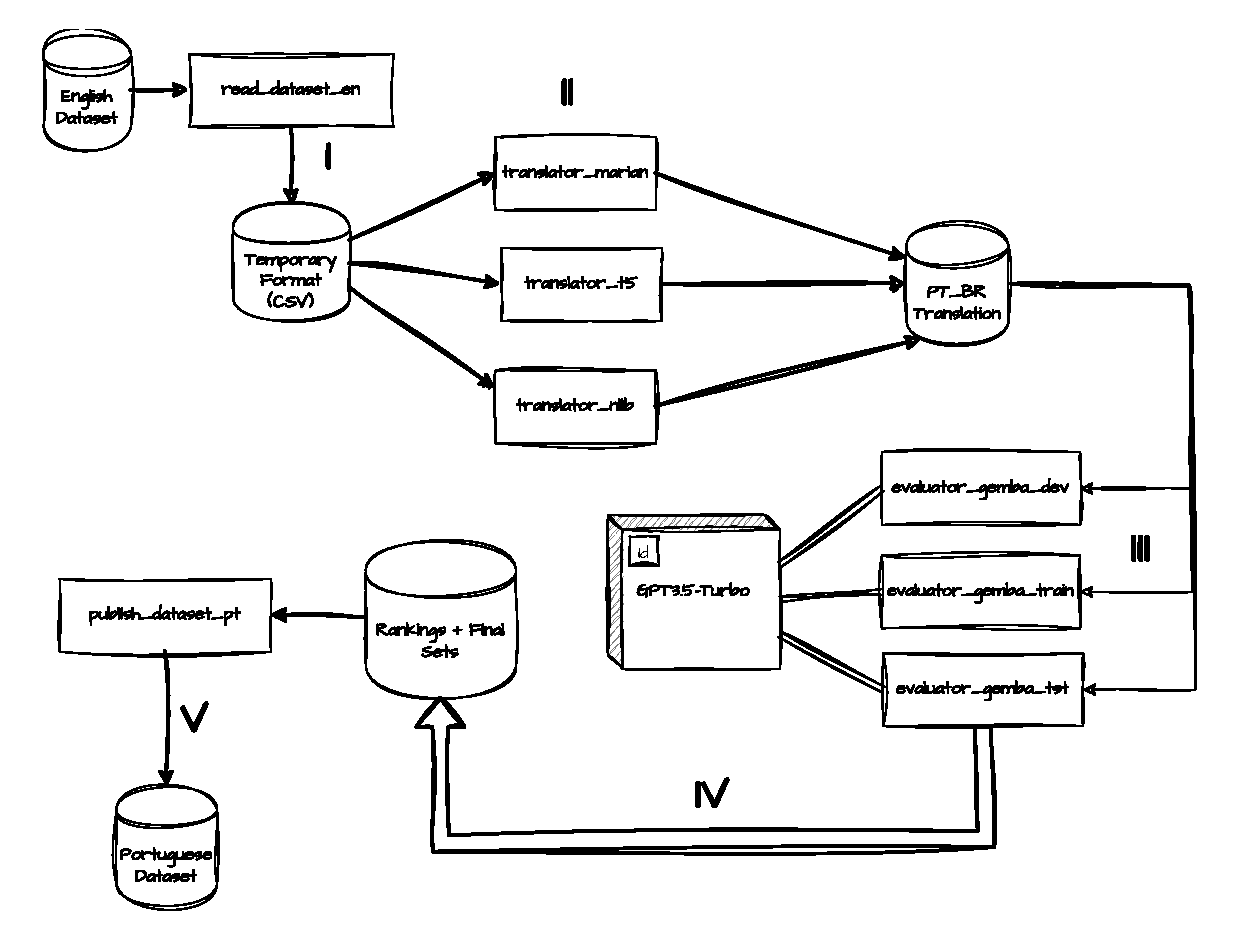
\includegraphics[width=0.90\textwidth]{drawio/translation.drawio.pdf}}
    \caption{Translation process including machine
    translation and GPT-based evaluation to select the best possible
    translation.}\label{fig:diagram}
\end{figure}
\FloatBarrier

\section{Results}

We have compared the outcomes of the translations methods using the GEMBA method. We discuss the results in the next sub-sections.

\subsection{Selected Translations per Model}

As can be seen on Figure \ref{fig:pie}, the model we selected most of our
translations from was the NLLB 1.3b from Meta. We believe this is due to the
fact that the strengths of this model lie on the translations of short
sentences. It is worthy noting that this is the model that uses the most
computing resources from the group of tested methods (around 6 Gbytes of GPU RAM).
Another conclusion from this chart is that even though NLLB 1.3b has the most
selected translations, there are still about 20\% of all translations being
selected from the other machine translation models.

\begin{figure}[htbp]
    \centering
    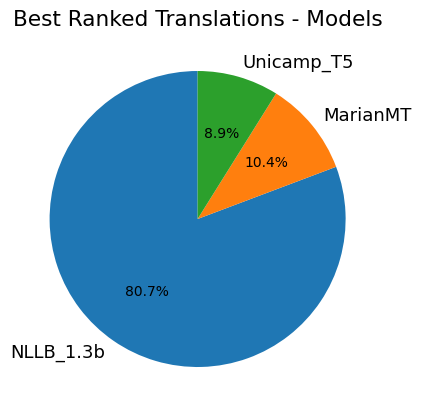
\includegraphics[width=0.4\textwidth]{figures/pie-chart.png}
    \caption{Selected Translations per Model.}\label{fig:pie}
\end{figure}
\FloatBarrier

\subsection{Kernel Density Estimates}

Figure \ref{fig:kde} shows a plot with the Kernel Density Estimates for the
distribution of the ratings for each model. We notice that, from the machine
translation models, NLLB 1.3b has the most evaluations towards the largest
evaluations, while the T5 model has a more flat distribution and Marian MT falls
in the middle.

\begin{figure}[htbp]
    \centering
    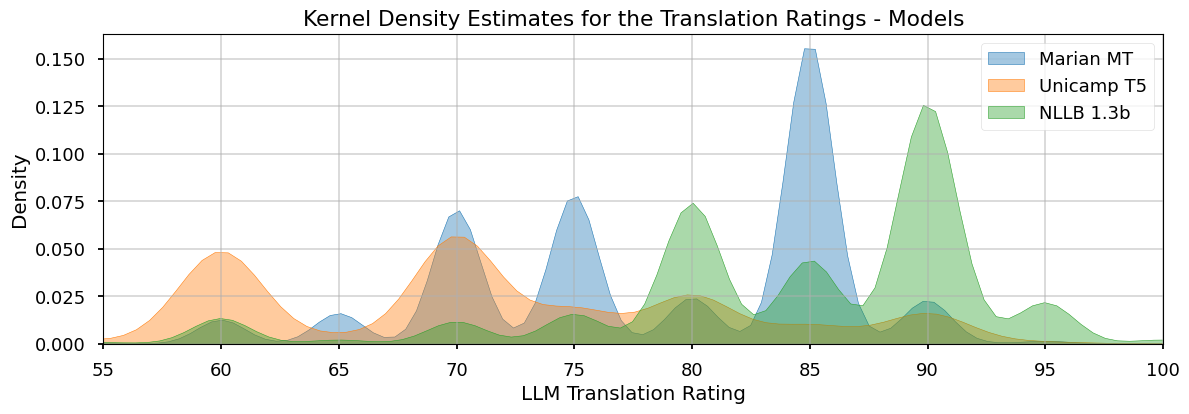
\includegraphics[width=0.9\textwidth]{figures/kde.png}
    \caption{KDE distributions per Model.}\label{fig:kde}
\end{figure}
\FloatBarrier

\subsection{Ratings per Sequence Length}

We proceed then to evaluate the impact of sequence length on the translation
quality in Figure \ref{fig:line-chart}. The graph compares the rating obtained
by each row of the original English dataset with the number of tokens of the
bundled sequence of strings. 

There is some ripple on the evaluation rating for larger sequences, but we did
not notice appreciable difference among the machine translation models.

\begin{figure}[htpb]
    \centering
    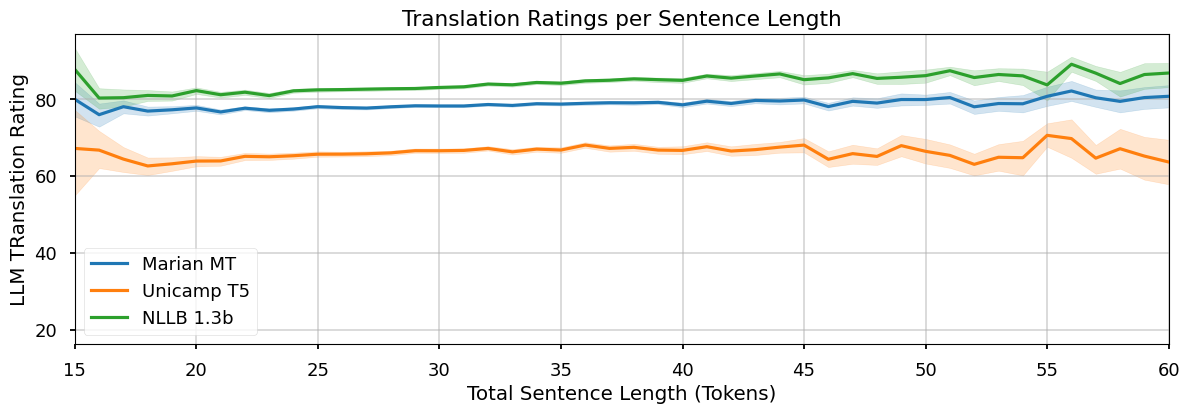
\includegraphics[width=0.9\textwidth]{figures/line-chart.png}
    \caption{Rating per Sequence Length per Model.}\label{fig:line-chart}
\end{figure}

\section{Conclusion and Future Work}

This paper presents a novel methodology to evaluate and select translations of sentences to compose a new dataset in the Portuguese language with minimal human effort making use of readily available machine translation models and API access to commercial large language models.

We evaluated different machine translation methods available at Hugging Face that produce similar, yet distinct enough output to allow for a comparison of quality with low cost incurred in the process.

The results demonstrated that more recent models such as the NLLB from Meta, even with support for multiple languages, tend to perform better than specialized models we had access to.

The Portuguese language dataset was published at Hugging face at \cite{socialiqa_pt}. 

We should also note here some advantages and difficulties we found during the conduction of this work. First, machine translation models with low hardware requirements were necessary enablers for this work. All the translations were performed locally with a consumer-grade graphics card with 16Gb of video RAM.
The usage of the GPT-3.5-turbo API in 2024 for a comparatively large dataset (38k lines) was only feasible due the low cost. For the translation evaluation,
over 50 thousand requests and 16 million tokens were sent using the Open AI API at an estimated total cost of less than US\$ 10. It is worth noting, however, that Open AI API speed was quite slow requiring over 50 hours for the whole
process.

We acknowledge, also, that this effort has limitations, since common-sense reasoning is heavily influenced by the differences between the cultural background, values, and experiences that can shape perspectives and the process of decision making inherent to the dataset we aimed to translate.

As future work, a thorough evaluation of the resulting dataset will be required to remove mistakes from the translation process. We note also that due to
the fact we discussed above that common-sense reasoning being very sensitive to cultural differences, a review of the dataset by Portuguese language speakers would be extremely valid for improving the quality of the translation results.

\section*{Declaration of Generative AI and AI-assisted technologies in the writing process}

During the preparation of this paper, the authors used ChatGPT to check the grammar and semantics of the human written text. After using this tool/service, the authors reviewed and edited the content as needed and take full responsibility for the content of the publication.

\begin{thebibliography}{8}
\bibitem{choi2022curious}Choi, Y. The curious case of commonsense intelligence. {\em Daedalus}. \textbf{151}, 139-155 (2022)
\bibitem{costa2022no}Costa-jussà, M., Cross, J., Çelebi, O., Elbayad, M., Heafield, K., Heffernan, K., Kalbassi, E., Lam, J., Licht, D., Maillard, J. \& Others No language left behind: Scaling human-centered machine translation. {\em ArXiv Preprint ArXiv:2207.04672}. (2022)
\bibitem{ghafoor2021impact}Ghafoor, A., Imran, A., Daudpota, S., Kastrati, Z., Batra, R., Wani, M. \& Others The impact of translating resource-rich datasets to low-resource languages through multi-lingual text processing. {\em IEEE Access}. \textbf{9} pp. 124478-124490 (2021)
\bibitem{kocmi2023large}Kocmi, T. \& Federmann, C. Large language models are state-of-the-art evaluators of translation quality. {\em ArXiv Preprint ArXiv:2302.14520}. (2023)
\bibitem{krause2023commonsense}Krause, S. \& Stolzenburg, F. Commonsense Reasoning and Explainable Artificial Intelligence Using Large Language Models. {\em European Conference On Artificial Intelligence}. pp. 302-319 (2023)
\bibitem{lee2023survey}Lee, S., Lee, J., Moon, H., Park, C., Seo, J., Eo, S., Koo, S. \& Lim, H. A survey on evaluation metrics for machine translation. {\em Mathematics}. \textbf{11}, 1006 (2023)
\bibitem{lopes2020lite}Lopes, A., Nogueira, R., Lotufo, R. \& Pedrini, H. Lite training strategies for Portuguese-English and English-Portuguese translation. {\em ArXiv Preprint ArXiv:2008.08769}. (2020)
\bibitem{sap2019socialiqa}Sap, M., Rashkin, H., Chen, D., LeBras, R. \& Choi, Y. Socialiqa: Commonsense reasoning about social interactions. {\em ArXiv Preprint ArXiv:1904.09728}. (2019)
\bibitem{socialiqa}AI, A. Social IQA. (https://allenai.org/data/socialiqa,2019), Accessed: 06/30/2024
\bibitem{socialiqa_pt}\blackout{Grassiotto, F. SocialIQa dataset v1.4 (PT) at Hugging Face. (https://huggingface.co/datasets/fabiogr/social\_i\_qa\_pt,2024), Accessed: 06/30/2024}
\bibitem{tiedemann2020opus}Tiedemann, J. \& Thottingal, S. OPUS-MT–building open translation services for the world. {\em Proceedings Of The 22nd Annual Conference Of The European Association For Machine Translation}. pp. 479-480 (2020)
\bibitem{freitag2021experts}Freitag, M., Foster, G., Grangier, D., Ratnakar, V., Tan, Q. \& Macherey, W. Experts, errors, and context: A large-scale study of human evaluation for machine translation. {\em Transactions Of The Association For Computational Linguistics}. \textbf{9} pp. 1460-1474 (2021)
\bibitem{mathur2020tangled}Mathur, N., Baldwin, T. \& Cohn, T. Tangled up in BLEU: Reevaluating the evaluation of automatic machine translation evaluation metrics. {\em ArXiv Preprint ArXiv:2006.06264}. (2020)
\bibitem{papineni2002bleu}Papineni, K., Roukos, S., Ward, T. \& Zhu, W. Bleu: a method for automatic evaluation of machine translation. {\em Proceedings Of The 40th Annual Meeting Of The Association For Computational Linguistics}. pp. 311-318 (2002)
\bibitem{snover2006study}Snover, M., Dorr, B., Schwartz, R., Micciulla, L. \& Makhoul, J. A study of translation edit rate with targeted human annotation. {\em Proceedings Of The 7th Conference Of The Association For Machine Translation In The Americas: Technical Papers}. pp. 223-231 (2006)
\bibitem{popovic2015chrf}Popović, M. chrF: character n-gram F-score for automatic MT evaluation. {\em Proceedings Of The Tenth Workshop On Statistical Machine Translation}. pp. 392-395 (2015)
\bibitem{lo2019yisi}Lo, C. YiSi-a unified semantic MT quality evaluation and estimation metric for languages with different levels of available resources. {\em Proceedings Of The Fourth Conference On Machine Translation (Volume 2: Shared Task Papers, Day 1)}. pp. 507-513 (2019)
\bibitem{chen2016enhanced}Chen, Q., Zhu, X., Ling, Z., Wei, S., Jiang, H. \& Inkpen, D. Enhanced LSTM for natural language inference. {\em ArXiv Preprint ArXiv:1609.06038}. (2016)
\bibitem{socialiqa_pt_impl} Anonymous Repository for the Social IQA translation project to Portuguese language. (https://anonymous.4open.science/r/SocialIQA\_pt-CB4F/README.md), Accessed: 06/30/2024
\end{thebibliography}

\end{document}
